\documentclass{article}
\usepackage[utf8]{inputenc}
\usepackage[spanish]{babel}
\usepackage{listings}
\usepackage{graphicx}
\usepackage[margin=2cm]{geometry}
\usepackage{color} %red, green, blue, yellow, cyan, magenta, black, white
\definecolor{mygreen}{RGB}{28,172,0} % color values Red, Green, Blue
\definecolor{mylilas}{RGB}{170,55,241}
\setlength{\parskip}{\baselineskip}

\let\oldsection\section
\renewcommand\section{\clearpage\oldsection}

\newcommand{\fref}[1]{figura \ref{fig:#1}}
\newcommand{\cref}[1]{cuadro \ref{table:#1}}
\newcommand{\sej}[1]{\subsection{Ejercicio #1}}

\lstset{language=Matlab,%
    %basicstyle=\color{red},
    basicstyle=\tt,
    breaklines=true,%
    morekeywords={matlab2tikz},
    keywordstyle=\color{blue},%
    morekeywords=[2]{1}, keywordstyle=[2]{\color{black}},
    identifierstyle=\color{black},%
    stringstyle=\color{mylilas},
    commentstyle=\color{mygreen},%
    showstringspaces=false,%without this there will be a symbol in the places where there is a space
    numbers=left,%
    numberstyle={\small \color{black}},% size of the numbers
    numbersep=9pt, % this defines how far the numbers are from the text
    emph=[1]{for,end,break},emphstyle=[1]\color{red}, %some words to emphasise
    %emph=[2]{word1,word2}, emphstyle=[2]{style},    
}

\begin{document}
\title{Prácticas de soldadura con un robot Puma560}
\author{Alejandro Adán Navarro \\ Alberto López Sánchez}
\date{marzo y abril de 2017}

\maketitle
\begin{center}
Robótica (GEI) · FIB · UPC
\end{center}
\clearpage
\tableofcontents
\clearpage
\listoffigures

\section{Introducción}

En esta memoria vamos a mostrar cómo hemos realizado las prácticas de laboratorio de la primera parte del curso (de la práctica 2 a la 6). Para ello usaremos explicaciones, códigos e imágenes.


Las prácticas de la primera parte del curso han consistido en utilizar un simulador de un Puma560 con el que hemos trabajado las transformaciones (traslaciones y rotaciones) y las interpolaciones, tanto de ángulos como de matrices homogéneas. 


A lo largo del curso, en las diferentes prácticas, hemos trabajado cada uno de los temas anteriores y, para acabar de sintetizarlo todo, hemos realizado un proyecto final donde programamos el robot para una tarea de soldadura.

\section{Práctica 2}
\subsection{Introducción}

El objetivo de esta sesión es empezar a trabajar con
orientaciones en 3D y empezar a ver la Robotics Toolbox. Para eso usaremos un sensor acelerómetro de 3 ejes encapsulado en una bola poliédrica (\fref{imagen_bola}).

\begin{figure}[h]
\centering
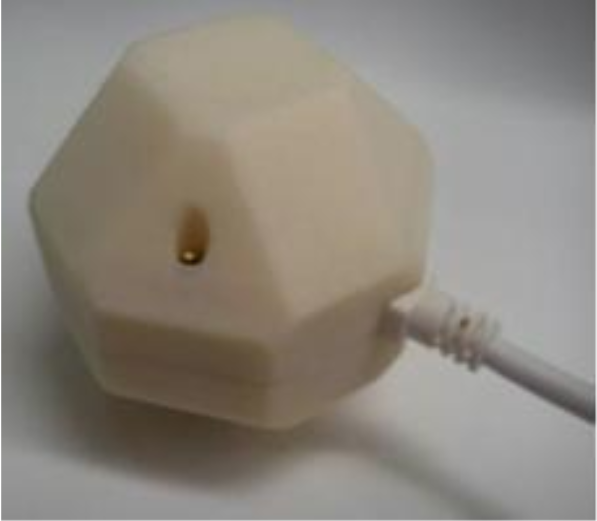
\includegraphics[width=0.5\textwidth]{bola.PNG}
\caption{Cubierta poliédrica del acelerómetro}
\label{fig:imagen_bola}
\end{figure}

\subsection{Configuración del entorno de trabajo}
Primeramente hemos instalado los controladores. Para comprobar que
estuvieran bien instalados, hemos usado el programa que viene incluido
con el driver.

Una vez comprobado que el acelerómetro funciona correctamente, 
hemos instalado las bibliotecas Robotics Toolbox.

\sej{1}

Primeramente hemos probado la Robotics Toolbox mostrando los ejes
de coordenadas. Para ello, hemos usado el siguiente código:

\begin{lstlisting}[frame=single]
trplot(eye(3))
\end{lstlisting}

Podemos ver el resultado en la \fref{ejcoor}.
\begin{figure}[h]
\centering
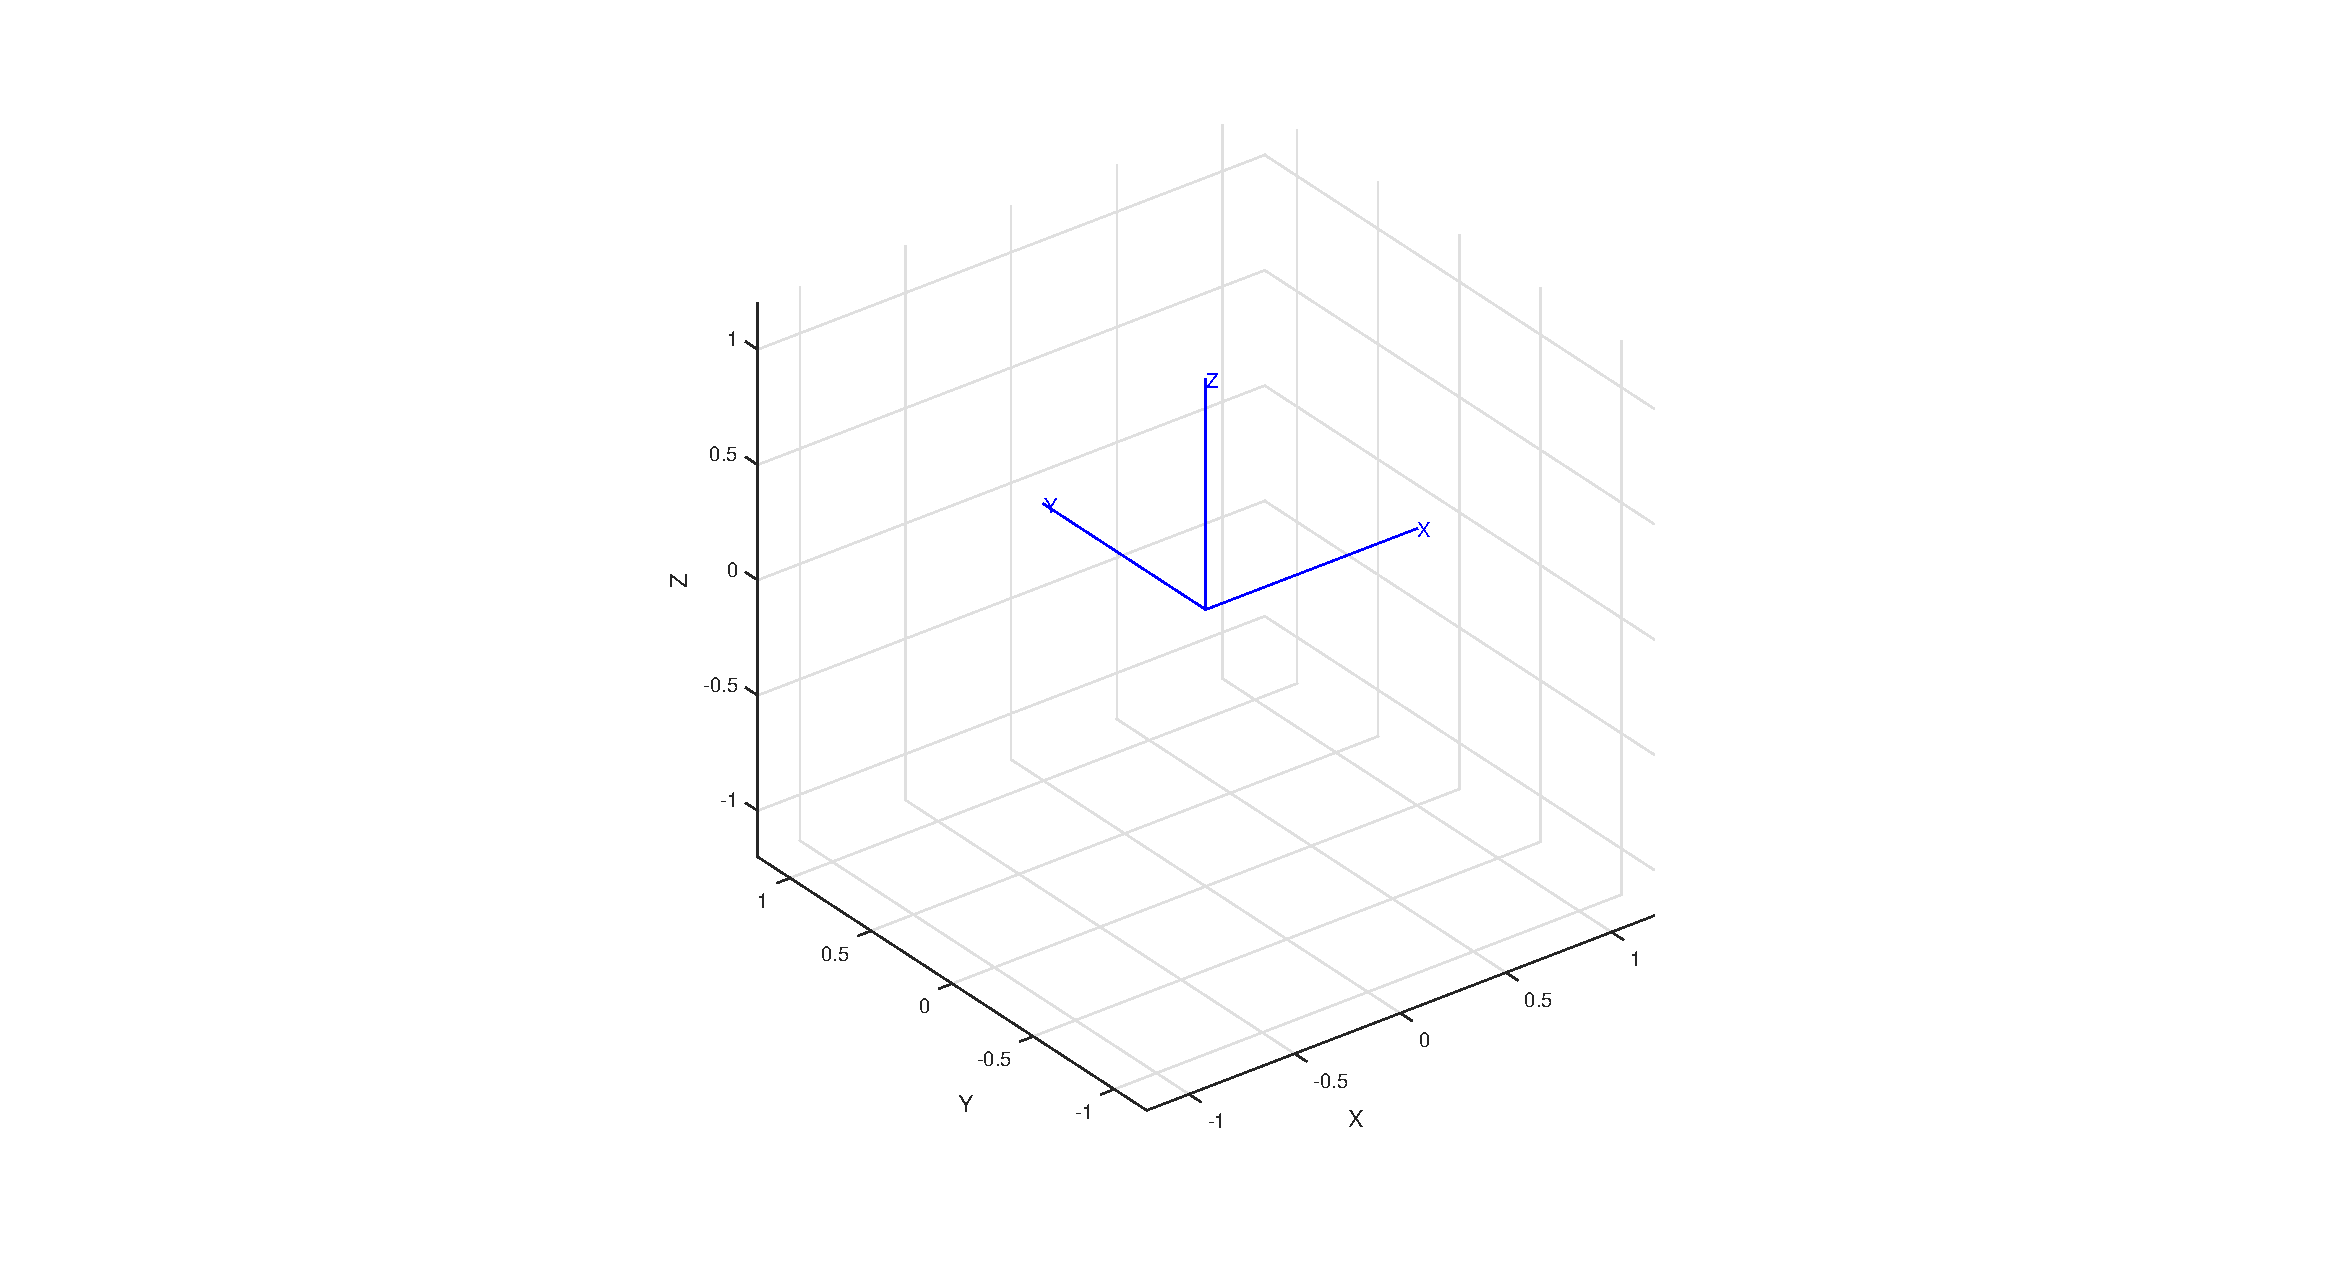
\includegraphics[width=0.8\textwidth]{practica2_ex1.eps}
\caption{Mostrando unos ejes de coordenadas (ejercicio 1)}
\label{fig:ejcoor}
\end{figure}

\sej{2}
Después hemos probado a mostrar una flecha en 3 dimensiones (véase la \fref{flecha3d}),
empleando este código:

\begin{lstlisting}[frame=single]
arrow3([0 0 0],[1 1 1]);
\end{lstlisting}

\begin{figure}[h]
\centering
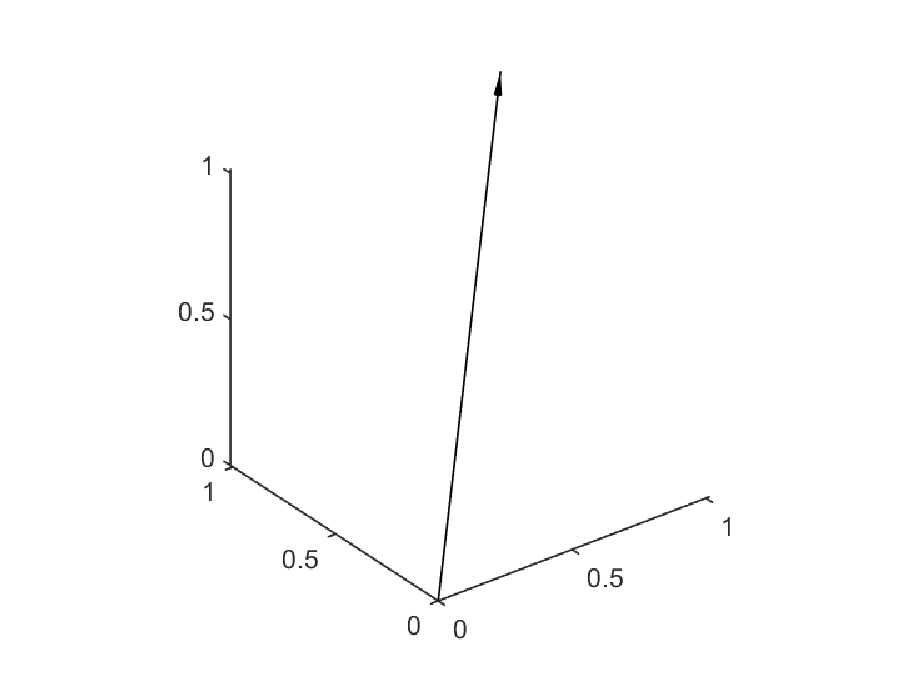
\includegraphics[width=0.8\textwidth]{practica2_ex3.eps}
\caption{Flecha en 3D (práctica 2, ejercicio 2)}
\label{fig:flecha3d}
\end{figure}

\sej{3}
A continuación, hemos utilizado el fichero {\tt read\_phidget\_sensor.m}
para leer los valores del acelerómetro.

\begin{lstlisting}[frame=single]
read_phidget_sensor()
\end{lstlisting}

El código anterior nos deja en el {\it workspace} los valores leídos, en la variable {\tt acceleration}.

\sej{4}
A partir de lo hecho, 
solamente necesitamos obtenerlos y ponerlos en un gráfico para 
ver la aceleración que sufre la bola.

El código que hemos usado para ello es el siguiente:
\begin{lstlisting}[frame=single]
read_phidget_sensor()
%acceleration = [0.5 0.2 0.7];
plot3([0,acceleration(1)],[0,acceleration(2)],[0,acceleration(3)])
axis([-2 2 -2 2 -2 2])

grid on
\end{lstlisting}

El resultado se puede ver en la \fref{grafacel}.
\begin{figure}[h]
\centering
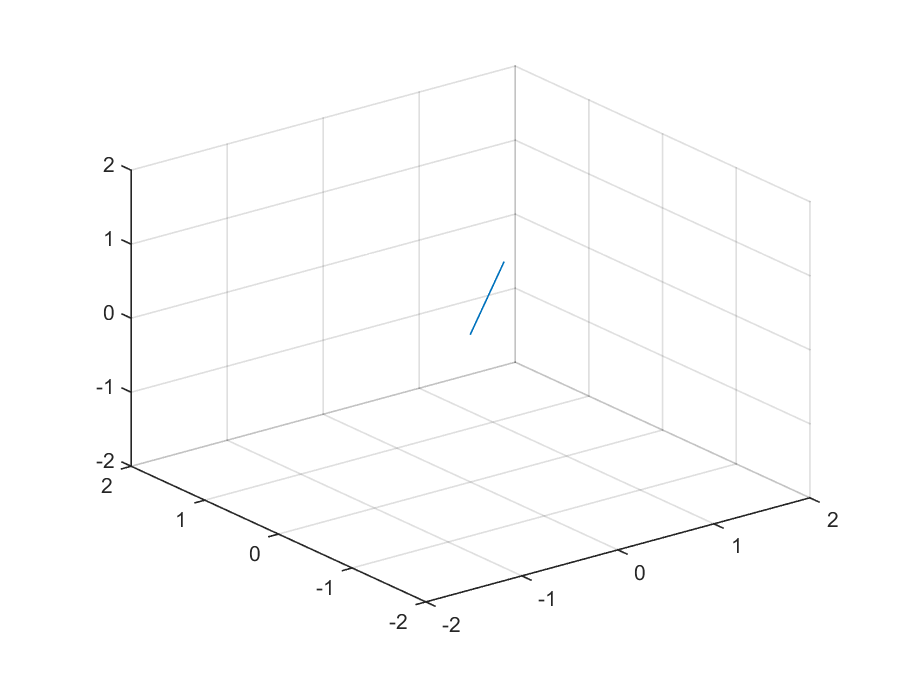
\includegraphics[width=0.8\textwidth]{practica2_ex4.eps}
\caption{Gráfico de la aceleración de la bola (práctica 2, ejercicio 4)}
\label{fig:grafacel}
\end{figure}

\sej{5}
Se nos pide demostrar por qué, si $(x,y,z)$ son las coordenadas de un punto en una superficie esférica de radio unidad y $(x,y)$ son las de su proyección 
en el plano $XY$, se cumple lo siguiente:
\[ (X,Y) = \left(\frac{x}{1-z},\frac{y}{1-z}\right) \]
\[ (x,y,z) = \left(\frac{2 X}{1+X^2+Y^2},\frac{2 Y}{1+X^2+Y^2},\frac{-1+X^2+Y^2}{1+X^2+Y^2}\right) \]

Trataremos primero la primera fórmula.

En caso de que $z$ fuera cero, se trataría de puntos que pertenecen a la vez a la superficie esférica y al plano (están a altura cero) y, por lo tanto, sabríamos que $X=x$ e 
$Y=y$ (la proyección de puntos de un plano sobre éste son ellos mismos). Como $1-z=1$ si $z=0$ y dividir un valor entre uno no lo cambia, tenemos que 
$X=x=\frac{x}{1}=\frac{x}{1-z}$ y $Y=y=\frac{y}{1}=\frac{y}{1-z}$.

En caso de que $z$ fuera uno, se trataría del cénit de la esfera, que se proyecta en el infinito. Por ello, como $1-z=0$ si $z=1$ y $\frac{x}{0}=\frac{y}{0}=\infty$, 
$X=\infty=\frac{x}{1-z}$ y $Y=\infty=\frac{y}{1-z}$.

En caso contrario, los puntos $(0,0,0)$, $(0,0,1)$ y $(X,0,0)$ forman un triángulo y los puntos $(x,0,0)$, $(x,0,z)$ y $(X,0,0)$ forman uno homotético (es decir,
con lados proporcionales a los del primero). Debido a esto, sabemos que $X$ es a 1 lo que $X-x$ es a $z$ ($\frac{X}{1}=\frac{X-x}{z}$), con lo que $X \cdot z = X - x$, $X \cdot
(z-1) = -x$ y finalmente $X = \frac{-x}{z-1} = \frac{x}{1-z}$. Las divisiones empleadas en esta demostración producen resultados finitos porque $z$ no es ni 0 ni 1. 

Por simetría, el mismo razonamiento es aplicable respecto a la relación entre $y$ e $Y$.

Ahora nos ocuparemos de la segunda, más complicada.

Sabemos que $X=\frac{x}{1-z}$, así que $x=X \cdot (1-z)$. Como $x^2+y^2+z^2=1$, $(X \cdot (1-z))^2+(Y \cdot (1-z))^2+z^2=1$, $(X^2+Y^2) \cdot (1-z)^2 + z^2 = 1$,
$(X^2+Y^2) \cdot (z^2 - 2\cdot z + 1) + z^2 = 1$ (porque $(1-z)^2=1^2-2\cdot 1 \cdot z + z^2 = z^2 - 2\cdot z + 1$), $(X^2+Y^2+1) \cdot z^2 - 2 \cdot (X^2+Y^2) \cdot z + 
(X^2+Y^2-1)= 0$. Debemos emplear aquí la fórmula para las ecuaciones de 2º grado para $b$ par ($x=\frac{-\frac{b}{2}\pm\sqrt{(\frac{b}{2})^2-ac}}{a}$):
$z = \frac{(X^2+Y^2)\pm\sqrt{(X^2+Y^2)^2-(X^2+Y^2+1) \cdot (X^2+Y^2-1)}}{X^2+Y^2+1}$.

Simplificamos el radicando: $(X^2+Y^2)^2-(X^2+Y^2+1) \cdot (X^2+Y^2-1)$,
$(X^4 + 2 \cdot X^2 \cdot Y^2 + Y^4) - (X^4+X^2 Y^2-X^2+Y^2 X^2+Y^4-Y^2+X^2+Y^2-1)$, $X^4 + 2 \cdot X^2 \cdot Y^2 + Y^4 - X^4-X^2 Y^2+X^2-Y^2 X^2-Y^4+Y^2-X^2-Y^2+1)$,
$X^4 - X^4 + 2 X^2 Y^2 - X^2 Y^2 - X^2 Y^2 + Y^4 - Y^4 + X^2 - X^2 + Y^2 - Y^2 + 1$, $1$. Así, la fórmula queda de este modo: $z = \frac{(X^2+Y^2)\pm\sqrt{1}}{X^2+Y^2+1}$.

Parece que tenemos dos posibles soluciones, pero la solución con $+$ es, en realidad, $z=1$, lo que es imposible porque el punto con $z=1$ es el cénit de la esfera y 
se proyecta en el infinito. Por lo tanto, nos queda solamente la solución con $-$, $z = \frac{X^2+Y^2-1}{X^2+Y^2+1}$, que es la dada.

Sabemos que $x=X \cdot (1-z)$ y que $z = \frac{X^2+Y^2-1}{X^2+Y^2+1}$, así que $x = X \cdot \left(1-\frac{X^2+Y^2-1}{X^2+Y^2+1}\right)$.
Si movemos el uno dentro de la fracción, nos queda $x = X \cdot \frac{(X^2+Y^2+1)-(X^2+Y^2-1)}{X^2+Y^2+1}$. Simplificamos el numerador y tenemos 
$x = X \cdot \frac{2}{X^2+Y^2+1}$. Movemos $X$ al numerador y obtenemos $x=\frac{2X}{X^2+Y^2+1}$, que es lo que indica la fórmula.

Por simetría, el mismo razonamiento es aplicable respecto a $y$.

\sej{6}
Utilizando las fórmulas demostradas en el ejercicio anterior, hemos implementado un nivel digital, proyectando estereográficamente los datos leídos del acelerómetro.

\begin{lstlisting}[frame=single]
trplot(eye(3))

while 1
    read_phidget_sensor()
    [x,y] = f1(acceleration(1),acceleration(2),acceleration(3));
    hold on
    line([0 x],[0 0], [0 y])
    hold off
    axis([-2 2 -2 2 -2 2])
    pause(1)
    % grid on
end
\end{lstlisting}

La función {\tt f1} es la que tiene el código que realiza la proyección y es el siguiente:

\begin{lstlisting}[frame=single]
function [x,y] = f1(x1,y1,z1)
    x = (x1/(1-z1));
    y = (y1/(1-z1));
end
\end{lstlisting}

\sej{7}

Nos piden que calculemos una matriz de rotación que, aplicada a un vector de aceleración, nos de un sistema de referencia.

La solución no es única pero, mientras mantengamos las relaciones $a = n \times o$, $n = o \times a$, $o = a \times n$, podemos cambiar los vectores $n$ y $o$.

\begin{lstlisting}[frame=single]
close all
clear all

% Fijamos una aceleracion que sepamos como tiene que dar el sistema de 
% referencia o cogemos los valores del sensor.
read_phidget_sensor()
%acceleration = [1/sqrt(3) 1/sqrt(3) 1/sqrt(3)];
acceleration = normc(acceleration);

c = normc([-acceleration(2);acceleration(1);0]);

n = normc(cross(c,acceleration));
mat = [n(1) c(1) acceleration(1)
       n(2) c(2) acceleration(2)
       n(3) c(3) acceleration(3)
    ];


trplot(mat);
\end{lstlisting}

¿Los tres vectores anteriores representan un sistema de referencia válido? Si, como podemos ver en la \fref{practica2_ex7}. porque son ortogonales entre sí y están normalizados.

\begin{figure}[h]
\centering
\includegraphics[width=0.8\textwidth]{practica2_ex7.eps}
\caption{En un primer momento del recorrido}
\label{fig:practica2_ex7}
\end{figure}


Para un vector aceleración de la forma $(a_x, a_y, a_z)$ la siguiente matriz nos proporciona el sistema de referencia: 
\[
M_{rot} = \left(
\begin{array}{ccc}
a_x*a_z        & -a_y & a_x  \\
a_y*a_z        & a_x  & a_y  \\
-a_x^2 - a_y^2 & 0    & a_z  \\
\end{array}
\right)
\]

\sej{8}

Nos piden que calculemos el eje equivalente de rotación y lo mostremos en el {\tt plot} según movemos la bola. Para ello, hemos añadido el siguiente código:

\begin{lstlisting}[frame=single]
[th_ta, v] = tr2angvec(mat);
line([0 v(1)], [0 v(2)], [0 v(3)]);

drawnow;
\end{lstlisting}

Podemos ver el resultado en la \fref{practica2_ex8}.

\begin{figure}[h]
\centering
\includegraphics[width=0.8\textwidth]{practica2_ex8.eps}
\caption{Sistema de referencia con el eje $z$ apuntando en la misma dirección que el vector de aceleración y eje equivalente de giro}
\label{fig:practica2_ex8}
\end{figure}


\section{Sesión 3}
\subsection{Introducción}
En esta sesión, hemos trabajado con un simulador en tres dimensiones del robot Puma560, con tal de poder representar en él varias configuraciones.

\subsection{Actividad 1}
En primer lugar, hemos probado el simulador con un conjunto de ángulos de giro de los seis ejes de los que dispone el robot. Así, hemos podido ver su funcionamiento (\fref{robotIni}).

\begin{figure}[h]
\centering
\includegraphics[width=0.8\textwidth]{practica3_ex1.eps}
\caption{El robot en posición inicial}
\label{fig:robotIni}
\end{figure}

\subsection{Actividad 2}

Hemos leído y entendido que hace cada parte del código. Para indicarlo aquí, le hemos añadido ciertos comentarios.

\begin{lstlisting}[frame=single]
function T06 = PlotPUMA560(angles)
%
% This function reads file 'linkdata.mat' containing the 3D models of the
% links of a PUMA560 and plots it with the joint angles given by 'angles'. 
% It returns the transformation that goes from the world reference frame to
% the tool reference frame.
%
% Author: F. Thomas (ESAII-UPC)
% Data: 02/28/2017
%
 
% Aqui carga los modelos 3D que representan al robot.
[linkdata]=load('linksdata.mat','s1','s2', 's3','s4','s5','s6','s7','A1');

% Aqui configura el espacio del plot.
range = [-1000 1000 -1000 1000 -1000 1000];

% Link parameters and joint angles
% Estos son los parametros Denavit-Hartenberg
a2 = 650;
a3 = 0;
d3 = 190;
d4 = 600;

% Angulos por defecto del robot.
%     Angle    Range                Default Name
%     Theta 1: 320 (-160 to 160)    90      Waist Joint
%     Theta 2: 220 (-110 to 110)    -90     Shoulder Joint
%     Theta 3: 270 (-135 to 135)    -90     Elbow Joint
%     Theta 4: 532 (-266 to 266)    0       Wrist Roll
%     Theta 5: 200 (-100 to 100)    0       Wrist Bend
%     Theta 6: 532 (-266 to 266)    0       Wrist Swival

% Los angulos que le hemos pasado a la funcion los convierte en radianes.
t = angles*pi/180; 

% Forward Kinematics (Cinematica directa)
% Calcula las diferentes matrices de transformacion para cada enlace del robot.
T01 = trotz(t(1));
T12 = trotx(-pi/2)*trotz(t(2));
T23 = transl(a2,0,d3)*trotz(t(3));

T34 = trotx(-pi/2)*transl(a3,0,d4)*trotz(t(4));
T45 = trotx(pi/2)*trotz(t(5));
T56 = trotx(-pi/2)*trotz(t(6));

T02 = T01*T12;
T03 = T02*T23;
T04 = T03*T34;
T05 = T04*T45;
T06 = T05*T56;

% Aqui calcula la transformacion de cada enlace.
Link1 = linkdata.s1.V1;
Link2 = linkdata.s2.V2*T01';
Link3 = linkdata.s3.V3*T02';
Link4 = linkdata.s4.V4*T03';
Link5 = linkdata.s5.V5*T04';
Link6 = linkdata.s6.V6*T05';
Link7 = linkdata.s7.V7*T06';

%%%%%%%%%%%%%%%%%%%%%%%%%%%%%%%%%%%%%%%%%%%%%%%%%%%%%%%%%%%%%
% Aqui dibuja el robot.
figure(1);
hold on;

L1 = patch('Faces', linkdata.s1.F1,...
           'Vertices', Link1(:,1:3),...
           'facec', [0.717,0.116,0.123],...
           'EdgeColor','none');
L2 = patch('Faces', linkdata.s2.F2,...
           'Vertices', Link2(:,1:3),...
           'facec', [0.216,1,0.583],...
           'EdgeColor','none');
L3 = patch('faces', linkdata.s3.F3,...
           'vertices', Link3(:,1:3),...
           'facec', [0.306,0.733,1],...
           'EdgeColor','none');
L4 = patch('faces', linkdata.s4.F4,...
           'vertices', Link4(:,1:3),...
           'facec', [1,0.542,0.493],...
           'EdgeColor','none');
L5 = patch('faces', linkdata.s5.F5,...
           'vertices' ,Link5(:,1:3),...
           'facec', [0.216,1,.583],...
           'EdgeColor','none');
L6 = patch('faces', linkdata.s6.F6,...
           'vertices' ,Link6(:,1:3),...
           'facec', [1,1,0.255],...
           'EdgeColor','none');
L7 = patch('faces', linkdata.s7.F7,...
           'vertices' ,Link7(:,1:3),...
           'facec', [1,1,0.255],...
           'EdgeColor','none');
       
% Hace el plot del sistema de coordenadas de la base.
trplot(eye(4),'length', 550, 'arrow');
% Hace el plot del sistema de coordenadas de la mano.
trplot(T06,'length', 550, 'arrow');

grid on;
axis(range);
daspect([1 1 1]);
view(3); 
camlight;
lighting gouraud;
%%%%%%%%%%%%%%%%%%%%%%%%%%%%%%%%%%%%%%%%%%%%%%%%%%%%%%%%%%%
\end{lstlisting}

\subsection{Actividad 3}
En esta tarea, debíamos decidir si el robot era desacoplado o no.

Vemos que si es desacoplado porque los 3 ejes de la muñeca interseccionan en un 
único punto. Esto significa que el movimiento de la muñeca solo cambia la orientación. 

\subsection{Actividad 4}
La actividad pide, con el objetivo de acelerar las animaciones, modificar la función que dibuja el robot para que no se vuelva a crear de nuevo el robot para cada pose, 
sino que se cree para la primera pose y más adelante solamente se actualicen las posiciones de los vértices de los modelos del robot con los nuevos ángulos.

\begin{lstlisting}[frame=single]
function T06 = simulador(angles)
%
% This function reads file 'linkdata.mat' containing the 3D models of the
% links of a PUMA560 and plots it with the joint angles given by 'angles'. 
% It returns the transformation that goes from the world reference frame to
% the tool reference frame.
%
% Author: F. Thomas (ESAII-UPC)
% Data: 02/28/2017
%
 
persistent linkdata;

[linkdata] = load('linksdata.mat','s1','s2', 's3','s4','s5','s6','s7','A1');

range = [-2000 2000 -2000 2000 -2000 2000];

% Link parameters and joint angles

a2 = 650;
a3 = 0;
d3 = 190;
d4 = 600;

%     Angle    Range                Default Name
%     Theta 1: 320 (-160 to 160)    90      Waist Joint
%     Theta 2: 220 (-110 to 110)    -90     Shoulder Joint
%     Theta 3: 270 (-135 to 135)    -90     Elbow Joint
%     Theta 4: 532 (-266 to 266)    0       Wrist Roll
%     Theta 5: 200 (-100 to 100)    0       Wrist Bend
%     Theta 6: 532 (-266 to 266)    0       Wrist Swival

t = angles*pi/180; 

% Forward Kinematics

T01 = trotz(t(1));
T12 = trotx(-pi/2)*trotz(t(2));
T23 = transl(a2,0,d3)*trotz(t(3));

T34 = trotx(-pi/2)*transl(a3,0,d4)*trotz(t(4));
T45 = trotx(pi/2)*trotz(t(5));
T56 = trotx(-pi/2)*trotz(t(6));

T02 = T01*T12;
T03 = T02*T23;
T04 = T03*T34;
T05 = T04*T45;
T06 = T05*T56;

Link1 = linkdata.s1.V1;
Link2 = linkdata.s2.V2*T01';
Link3 = linkdata.s3.V3*T02';
Link4 = linkdata.s4.V4*T03';
Link5 = linkdata.s5.V5*T04';
Link6 = linkdata.s6.V6*T05';
Link7 = linkdata.s7.V7*T06';

%%%%%%%%%%%%%%%%%%%%%%%%%%%%%%%%%%%%%%%%%%%%%%%%%%%%%%%%%%%%%
figure(1);
hold on;

persistent L1 L2 L3 L4 L5 L6 L7;
persistent h;
if isempty(L1) 
       L1 = patch('Faces', linkdata.s1.F1,...
           'Vertices', Link1(:,1:3),...
           'facec', [0.717,0.116,0.123],...
           'EdgeColor','none');   
       L2 = patch('Faces', linkdata.s2.F2,...
           'Vertices', Link2(:,1:3),...
           'facec', [0.216,1,0.583],...
           'EdgeColor','none');
        L3 = patch('faces', linkdata.s3.F3,...
           'vertices', Link3(:,1:3),...
           'facec', [0.306,0.733,1],...
           'EdgeColor','none');
        L4 = patch('faces', linkdata.s4.F4,...
           'vertices', Link4(:,1:3),...
           'facec', [1,0.542,0.493],...
           'EdgeColor','none');
        L5 = patch('faces', linkdata.s5.F5,...
           'vertices' ,Link5(:,1:3),...
           'facec', [0.216,1,.583],...
           'EdgeColor','none');
        L6 = patch('faces', linkdata.s6.F6,...
           'vertices' ,Link6(:,1:3),...
           'facec', [1,1,0.255],...
           'EdgeColor','none');
        L7 = patch('faces', linkdata.s7.F7,...
           'vertices' ,Link7(:,1:3),...
           'facec', [1,1,0.255],...
           'EdgeColor','none');
       

        h = trplot(eye(4),'length', 550, 'arrow');
        trplot(h, T06,'length', 550, 'arrow');

        grid on;
        axis(range);
        daspect([1 1 1]);
        view(3); 
        camlight;
        lighting gouraud;
else
        set(L1, 'Vertices', Link1(:,1:3))
        set(L2, 'Vertices', Link2(:,1:3))
        set(L3, 'Vertices', Link3(:,1:3))
        set(L4, 'Vertices', Link4(:,1:3))
        set(L5, 'Vertices', Link5(:,1:3))
        set(L6, 'Vertices', Link6(:,1:3))
        set(L7, 'Vertices', Link7(:,1:3))
        trplot(h, eye(4), 'length', 550, 'arrow');
        trplot(h, T06);
end 
%%%%%%%%%%%%%%%%%%%%%%%%%%%%%%%%%%%%%%%%%%%%%%%%%%%%%%%%%%%
\end{lstlisting}

\subsection{Actividad 5}
Se nos pide en este ejercicio que, en base a lo obtenido en el ejercicio anterior, reproduzcamos la animación mostrada en un fichero de vídeo que se nos hace llegar.

Esta animación realiza los movimientos siguientes:
\begin{itemize}
\item Giro de 180º a la izquierda en el primer eje
\item Giro de 180º a la derecha en el primer eje
\item Giro de 180º por arriba en el segundo eje
\item Giro de 180º por arriba en el segundo eje
\item Giro de 180º por fuera en el tercer eje
\item Giro de 180º por fuera en el tercer eje
\item Giro de 180º hacia la izquierda de la mano alrededor de su eje $Z$
\item Giro de 180º hacia la derecha de la mano alrededor de su eje $Z$
\item Giro de 180º de la mano por fuera alrededor de su eje $Y$
\item Giro de 180º de la mano por fuera alrededor de su eje $Y$
\item Giro de 180º hacia la izquierda de la pinza
\item Giro de 180º hacia la derecha de la pinza
\end{itemize}

\begin{lstlisting}[frame=single]
clear all
close all


for a = 0:180 % 1 ida
    simulador([a,0,0,0,0,0]);
    drawnow;
end
for b = 0:180 % 1 vuelta
    simulador([180-b,0,0,0,0,0]);
    drawnow;
end
for c = 0:180 % 1 subida
    simulador([0,-c,0,0,0,0]);
    drawnow;
end
for c = 0:180 % 1 bajada
    simulador([0,180+c,0,0,0,0]);
    drawnow;
end
for d = 0:180
    simulador([0,0,-d,0,0,0]);
    drawnow;
end
for d = 0:180
    simulador([0,0,180+d,0,0,0]);
    drawnow;
end
for e = 0:180
    simulador([0,0,0,-e,0,0]);
    drawnow;
end
for e = 0:180
    simulador([0,0,0,180+e,0,0]);
    drawnow;
end
for f = 0:180
    simulador([0,0,0,0,-f,0]);
    drawnow;
end
for f = 0:180
    simulador([0,0,0,0,180+f,0]);
    drawnow;
end
for g = 0:180
    simulador([0,0,0,0,0,-g]);
    drawnow;
end
for g = 0:180
    simulador([0,0,0,0,0,180+g]);
    drawnow;
end
\end{lstlisting}



\subsection{Actividad 6}
Aquí se nos dice que comprobemos que si cambiamos los ángulos de giro de los tres últimos ejes del robot por $\phi_4+\pi$, $-\phi_5$ y $\phi_6+\pi$ (siendo $\phi_4$, $\phi_5$
y $\phi_6$ los ángulos de los ejes 4, 5 y 6 de éste) el resultado es el mismo.

Para comprobar si esta propiedad es cierta, hemos hecho un código en el que se ve animado como cambia la posición de la mano partiendo de una ubicación aleatoria para acabar volviendo al mismo sitio donde empezó.

\begin{lstlisting}[frame=single]
clear all
close all

% Cogemos una posision aleatoria y verificamos la propiedad.
a = rand() * 180;
b = rand() * 180;
c = rand() * 180;

simulador([0,0,0,a,b,c]);

aP = a + 180;
bP = -b;
cP = c + 180;

i = a;
j = b;
k = c;

pause(3)
    

while i < aP || j > bP || k < cP
    if i < aP
        i = i + 1;
    end
    if j > bP
        j = j - 1;
    end
    if k < cP
        k = k + 1;
    end
    simulador([0,0,0,i,j,k]);
    drawnow;
end
\end{lstlisting}

La demostración de este hecho sigue.

Si consideramos que las rotaciones 4ª, 5ª y 6ª corresponden, respectivamente, a los ejes $x$, $y$ y $z$ de la muñeca del robot, al incrementar la 4ª rotación en $\pi$ radianes estamos colocando el eje $y$ en sentido opuesto al que tendría con la rotación original, lo que hace que, a su vez, se invierta el sentido (interpretado respecto a las coordenadas que había antes del 4º giro) de una rotación respecto a dicho eje.

Tras las rotaciones 4ª y 5ª, los ejes $x$ e $y$ quedan situados en sentido contrario al que tendrían ordinariamente en ese momento pero el eje $z$ no, con lo que hay que realizar una rotación de $\pi$ radianes alrededor del eje $z$ para que la rotación hecha sobre este eje acabe donde debe.

\section{Sesión 4}
\subsection{Introducción}
En esta sesión interpolamos los ángulos de giro del robot de forma lineal, para llegar de una configuración de ángulos a otra. Encontramos los parámetros Denavit-Hartenberg y creamos un robot con las herramientas de la Robotics Toolbox con estos parámetros.

\subsection{Implementar un planificador de caminos interpolando los ángulos de los motores}

\subsubsection{Generar dos juegos de ángulos aleatorios}
Hemos generado dos juegos de ángulos, tales que el robot pasara de unos a otros.

Juego origen:
\begin{lstlisting}[frame=single]
a = 0;
b = 0;
c = 0;
d = rand() * 180;
e = rand() * 180;
f = rand() * 180;
\end{lstlisting}

Juego destino:
\begin{lstlisting}[frame=single]
a1 = 90;
b1 = 180;
c1 = 0;
d1 = rand() * 180;
e1 = rand() * 180;
f1 = rand() * 180;
\end{lstlisting}

\subsubsection{Resolver la cinemática directa para los dos juegos de ángulos}
\begin{lstlisting}[frame=single]
t1 = simulador([a b c d e f]);
t2 = simulador([a1 b1 c1 d1 e1 f1]);
\end{lstlisting}

\subsubsection{Dibujar los ejes de referencia de los dos juegos de ángulos}
\begin{lstlisting}[frame=single]
trplot(t1,'length', 550, 'arrow');
trplot(t2,'length', 550, 'arrow');
\end{lstlisting}

\subsubsection{Generar el movimiento para que el robot conecte las dos configuraciones interpolando los ángulos de ejes}
\begin{lstlisting}[frame=single]
function r = ajustarp(a, a1, p)
   	r = a1*(p / 100) + a*(1-(p/100));
end
\end{lstlisting}

\begin{lstlisting}[frame=single]
for p = 0:0.01:100
    a = ajustarp(a,a1,p);
    b = ajustarp(b,b1,p);
    c = ajustarp(c,c1,p);
    d = ajustarp(d,d1,p);
    e = ajustarp(e,e1,p);
    f = ajustarp(f,f1,p);
   
    %disp(a);
    %disp(b);
    %disp(c);
    
    simulador([a,b,c,d,e,f]);
    drawnow;
end
\end{lstlisting}

\subsubsection{Dibujar la trayectoria seguida por el centro de la pinza}

En la \fref{lab4_b_5_1}, la \fref{lab4_b_5_2} y la \fref{lab4_b_5_3} podemos ver cómo se ha movido el robot.

\begin{figure}[h]
\centering
\includegraphics[width=0.8\textwidth]{lab4_b_5_1.eps}
\caption{El robot en un primer momento del recorrido}
\label{fig:lab4_b_5_1}
\end{figure}

\begin{figure}[h]
\centering
\includegraphics[width=0.8\textwidth]{lab4_b_5_2.eps}
\caption{El robot en un momento más avanzado del recorrido}
\label{fig:lab4_b_5_2}
\end{figure}

\begin{figure}[h]
\centering
\includegraphics[width=0.8\textwidth]{lab4_b_5_3.eps}
\caption{El robot al final del recorrido}
\label{fig:lab4_b_5_3}
\end{figure}

\subsection{Parámetros Denavit-Hartenberg}
\begin{table}[h]
\centering
\caption{Parámetros Denavit-Hartenberg generales para un Puma560}
\label{table:parametros_DH}
\begin{tabular}{l|llll}
Articulación & $\theta$   & $d_i$  & $a_i$   & $\alpha_i$ \\ \hline
1            & $\theta_1$ & $d_1$  & $0$     & $90$       \\
2            & $\theta_2$ & $d_2$  & $a_2$   & $0$         \\
3            & $\theta_3$ & $0$    & $-a_3$  & $-90$        \\
4            & $\theta_4$ & $d_4$  & $0$     & $90$       \\
5            & $\theta_5$ & $0$    & $0$     & $-90$       
\end{tabular}
\end{table}

\begin{table}[h]
\centering
\caption{Parámetros Denavit-Hartenberg calculados a partir del simulador proporcionado}
\label{table:parametros_DH2}
\begin{tabular}{l|llll}
Articulación & $\theta$   & $d_i$  & $a_i$   & $\alpha_i$ \\ \hline
1            & $\theta_1$ & $0$  & $0$     & $90$       \\
2            & $\theta_2$ & $0$  & $650$   & $0$         \\
3            & $\theta_3$ & $190$    & $0$  & $-90$        \\
4            & $\theta_4$ & $600$  & $0$     & $90$       \\
5            & $\theta_5$ & $0$    & $0$     & $-90$       
\end{tabular}
\end{table}

Podemos ver los parámetros genéricos en el \cref{parametros_DH} y los calculados en el \cref{parametros_DH2}.

\subsection{Implementar un robot con los mismos parámetros Denavit-Hartenberg usando las funciones de la Robotics Toolbox}

\begin{lstlisting}[frame=single]
close all
clear all

%pi = 3.141592;
L(1) = Link([0 0 0 pi/2]);
L(2) = Link([0 0 650 0]);
L(3) = Link([0 190 0 -pi/2]);
L(4) = Link([0 600 0 pi/2]);
L(5) = Link([0 0 0 -pi/2]);
L(6) = Link([0 0 0 0]);
Robot = SerialLink(L);

mdl_puma560;
Robot.plot([0 pi/2 pi/4 0 0 0], 'notiles');
simulador([0 -90 45 0 0 0]);
\end{lstlisting}

En la \fref{lab4_DH} podemos ver como se compara el resultado con nuestro simulador.

\begin{figure}[h]
\centering
\includegraphics[width=0.8\textwidth]{lab4_DH.eps}
\caption{Nuestro Simulador y el robot creado a partir de los parámetros DH}
\label{fig:lab4_DH}
\end{figure}

\subsection{Sustituir las matrices $T_{ij}$ en nuestro simulador por las correspondientes matrices Denavit-Hartenberg}

Para ello, hemos creado variables simbólicas y nos hemos quedado con cada matriz en cada punto de la multiplicación. Con ello, hemos obtenido el siguiente código.
\begin{lstlisting}[frame=single]
T01 = [cos(t(1)), -sin(t(1)), 0, 0;
       sin(t(1)), cos(t(1)), 0, 0; 
       0, 0, 1, 0; 
       0, 0, 0, 1];
T12 = [cos(t(2)), -sin(t(2)), 0, 0;
       0, 0, 1, 0; 
       -sin(t(2)), -cos(t(2)), 0, 0;
       0, 0, 0, 1];
T23 = [cos(t(3)), -sin(t(3)), 0, 650;
       sin(t(3)), cos(t(3)), 0, 0; 
       0, 0, 1, 190;
       0, 0, 0, 1];
T34 = [cos(t(4)), -sin(t(4)), 0, 0;
       0, 0, 1, 600;
       -sin(t(4)), -cos(t(4)), 0, 0;
       0, 0, 0, 1];
T45 = [ cos(t(5)), -sin(t(5)), 0, 0;
        0, 0, -1, 0;
        sin(t(5)), cos(t(5)), 0, 0;
        0, 0, 0, 1];
T56 = [cos(t(6)), -sin(t(6)), 0, 0;
       0, 0, 1, 0;
       -sin(t(6)), -cos(t(6)), 0, 0;
       0, 0, 0, 1];
\end{lstlisting}

\subsection{Descargar {\tt CreateScene.m} y ejecutarlo}
Esta tarea es el principio de la segunda parte de la práctica. Nos pide entender el fichero {\tt CreateScene.m} y ejecutarlo.

Este fichero crea un escenario con una plataforma de color rojo, en el lateral de la cual hay colocado un cilindro con una hélice alrededor, que debemos soldar al cilindro.

\subsection{Integrar elementos}
Ahora, se trata de integrar la plataforma y el cilindro con hélice con el robot en la misma escena. Para ello, hemos modificado tres líneas en nuestro simulador:
\begin{lstlisting}[frame=single]
T00 = transl(1000,-1000,1250);
\end{lstlisting}

\begin{lstlisting}[frame=single]
T01 = T00 * trotz(t(1));
\end{lstlisting}

\begin{lstlisting}[frame=single]
Link1 = linkdata.s1.V1*T00';
\end{lstlisting}

La primera es una línea que hemos añadido antes de la definición de {\tt T01}; las otras dos son modificaciones de las líneas que definen {\tt T01} y {\tt Link1}, respectivamente.

Con estos cambios ponemos el robot junto con la plataforma. Si lo pintamos todo junto, obtenemos el resultado que puede verse en la \fref{escsol}.

\begin{figure}[h]
\centering
\includegraphics[width=0.8\textwidth]{escenaSoldadura.eps}
\caption{Escena en la que se muestran la plataforma y el cilindro con hélice con el robot}
\label{fig:escsol}
\end{figure}

Pasamos a explicar el fichero (los comentarios con {\tt \%\%} son nuestros; los demás estaban en el fichero).
\begin{lstlisting}[frame=single]
%% Carga los ficheros del tubo y el espiral
%Loads the spiral model and translates and rotates it to its place
chapa = stlread('ChapaEspiral.stl');
aux = [chapa.vertices(:,1:3)'; ones(size(chapa.vertices(:,1)))'];
aux2 = (transl(750, -225, 850)*trotx(-20, 'deg')*aux)';
chapa.vertices = aux2(:,1:3);

%Loads the tube model and translates and rotates it to its place
tubo = stlread('Tubo.stl');
aux = [tubo.vertices(:,1)'; tubo.vertices(:,2)'; tubo.vertices(:,3)'; ones(size(tubo.vertices(:,1)))'];
aux2 = (transl(750, -225, 850)*trotx(-20, 'deg')*transl(100, 0, 100)*aux)';
tubo.vertices = aux2(:,1:3);

%% Define la plataforma
%%%% Definition of the Panel vertices and faces  
v1 = [0 0 0; 3000 0 0; 3000 0 200; 0 0 200; 3000 500 1700; ...
      0 500 1700; 3000 700 1700; 0 700 1700; 3000 700 0; ...
      0 700 0; 0 700 200; 3000 700 200];

f1 = [1 2 3 4; 4 3 5 6; 6 5 7 8; 8 7 9 10; 1 10 9 2; ...
      2 9 12 3; 3 12 7 5; 1 4 11 10; 4 6 8 11];

%% Define la base del robot
%%%% Definition of the Base vertices and faces 
v2 = [240 -1500 0; 2740 -1500 0; 2740 -1500 200; ...
    240 -1500 200; 2740 -500 200; 240 -500 200; ...
    2740 -500 0; 240 -500 0];
f2 = [1 2 3 4; 4 3 5 6; 6 5 7 8; 8 7 2 1; 2 7 5 3; 1 4 6 8];

%%%% Definition of a circle 
radius = 350;      
theta = linspace(0,2*pi);          
X = radius.*cos(theta);  
Y = radius.*sin(theta);  
C = trotx(70, 'deg')*transl(950, 950, 100)*[X; Y; zeros(size(X)); ones(size(X))];


%%%%%%%%%%%%%%%%%%%%%%%%%%%%%%%%%%%%%%%%%%%%%%%%%%%%%%%%%%%%%%%%%%%%%%%%%%%
%% Dibujarlo todo
%Plot the models

figure(2);

grid on;
axis([-1000 4000 -2000 1000 0 3000]);
daspect([1 1 1]);
view(3); 
camlight;
lighting gouraud;
hold on;

patch(chapa,'FaceColor',       [0.8 0.8 1.0], ...
         'EdgeColor',       'none',        ...
         'FaceLighting',    'gouraud',     ...
         'AmbientStrength', 0.15);

patch(tubo,'FaceColor',       [0.8 0.8 1.0], ...
         'EdgeColor',       'none',        ...
         'FaceLighting',    'gouraud',     ...
         'AmbientStrength', 0.15);
     
%material('dull');

patch('vertices',v1,'faces',f1,'facecolor','r'); 
patch('vertices',v2,'faces',f2,'facecolor','g');

fill3(H(1,:),H(2,:),H(3,:),'b');
\end{lstlisting}

\section{Sesión 5}
\subsection{Introducción}
En esta sesión resolveremos la cinemática inversa de nuestro Puma 560 y conseguiremos
que el robot trace una línea recta.

\subsection{Comprobación de la funcion IKPuma560}

\subsubsection{Resolver la cinemática directa para los ángulos $[0, 0, 0, 0, 0, 0]$}
\begin{lstlisting}[frame=single]
Torig = simulador([0,0,0,0,0,0]);
\end{lstlisting}

\subsubsection{Resolver la cinemática inversa para la transformación homogénea obtenida en el paso anterior, que tiene hasta 8 posibles combinaciones, y hacer un {\tt plot} de todas}

\begin{lstlisting}[frame=single]
close all
clear all
Torig = simulador([0,0,0,0,0,0]);

for i = -1:2:1
    for j = -1:2:1
        for k = -1:2:1
            angulos = PumaIK(Torig, i, j, k);
            simulador(angulos);
            drawnow;
            print(['pumaDos' i+49 j+49 k+49],'-depsc');
            pause(1);
        end
    end
end
\end{lstlisting}

Este código creará ficheros con nombres de la forma {\tt puma\{0,2\}\{0,2\}\{0,2\}.eps} en el directorio de trabajo, que contendrán las diferentes configuraciones del robot que
permiten llegar a la posición indicada (si las hay). En la \fref{pumaAll} podemos ver el resultado.

\begin{figure}[h]
\centering
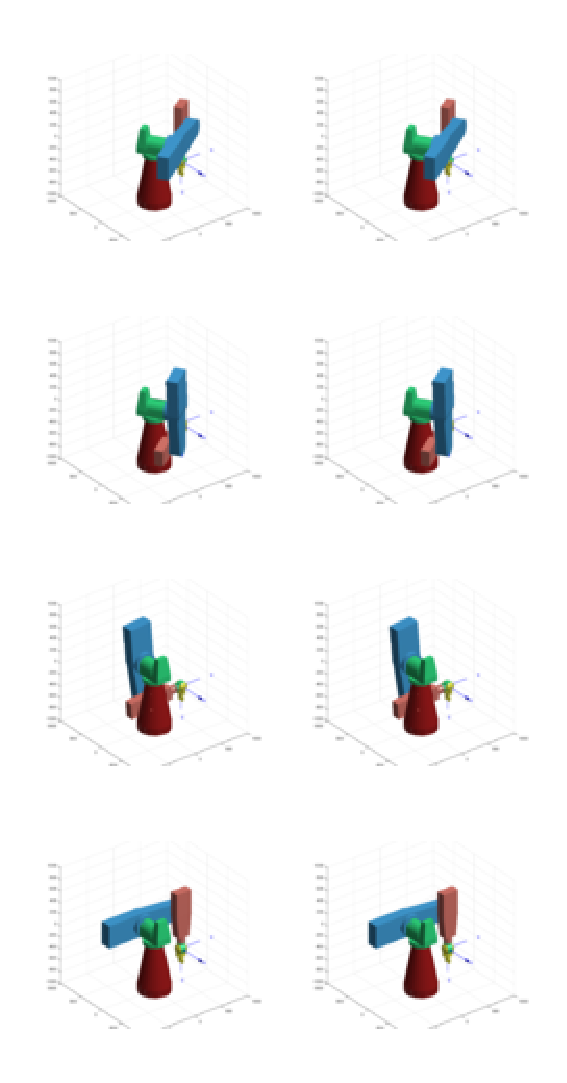
\includegraphics[width=0.5\textwidth]{montage.eps}
\caption{Primera configuración de ángulos con el plot de todas las opciones}
\label{fig:pumaAll}
\end{figure}


\subsubsection{Repetir la misma operación para un juego de ángulos diferentes}
Se trata del mismo código, pero sustituyendo la tercera línea por esta…
\begin{lstlisting}[frame=single]
Torig = simulador([90,0,0,0,0,0]);
\end{lstlisting}
…y la undécima por esta otra:
\begin{lstlisting}[frame=single]
            print(['pumaDos' i+49 j+49 k+49],'-depsc');
\end{lstlisting}

En la \fref{pumaDosAll} podemos ver el resultado.


\begin{figure}[h]
\centering
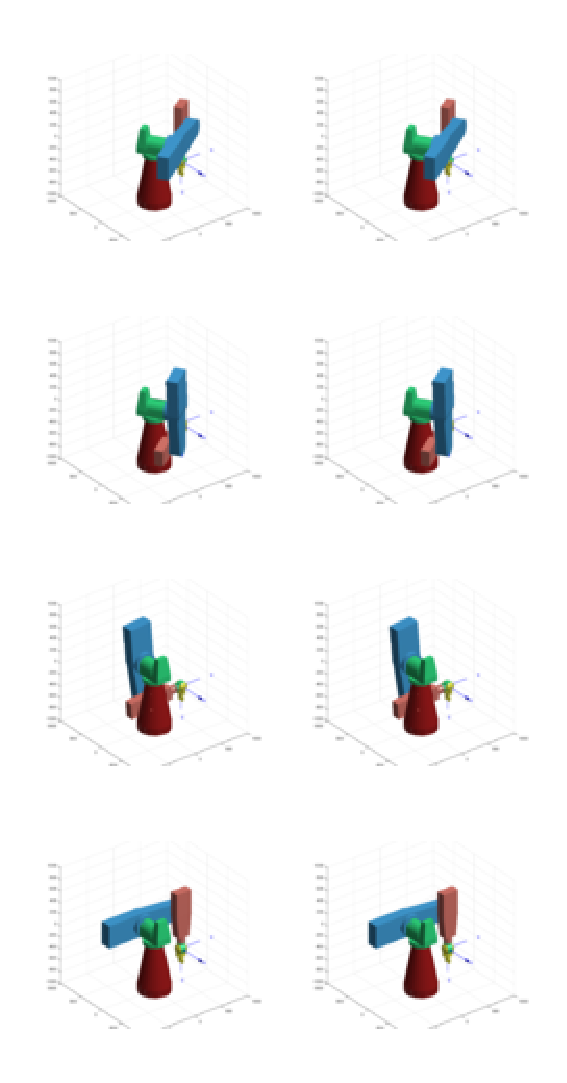
\includegraphics[width=0.5\textwidth]{montage.eps}
\caption{Segunda configuración de ángulos con el plot de todas las opciones}
\label{fig:pumaDosAll}
\end{figure}

\subsection{Interpolando ángulos con {\tt jtraj} y {\tt ctraj}}
Ahora vamos a ver los dos tipos de interpolación que podemos realizar.
\subsubsection{Interpolando ángulos con {\tt jtraj}}
Con {\tt jtraj} lo que hacemos es interpolar los ángulos de giro
para pasar de la posición inicial a la posición final.

Para ello hemos fijado dos juegos de ángulos: ángulos iniciales {\tt Torig} y ángulos destino {\tt Tdest}.

\begin{lstlisting}[frame=single]
Torig = [0,0,0,0,0,0];
Tdest = [90,-90,0,0,0,0];
\end{lstlisting}

Hemos calculado 100 pasos con los juegos de ángulos interpolados

\begin{lstlisting}[frame=single]
pasos = jtraj(Torig, Tdest, 100);
\end{lstlisting}

Finalmente ejecutamos el simulador para ver cómo quedan. El resultado se puede ver en la \fref{lab5jtraj}.
\begin{lstlisting}[frame=single]
for i = 1:100
    simulador(pasos(i,:));
    drawnow;
end
\end{lstlisting}

\begin{figure}[h]
\centering
\includegraphics[width=0.5\textwidth]{lab5jtraj.eps}
\caption{Resultado de la interpolación con {\tt jtraj}}
\label{fig:lab5jtraj}
\end{figure}

\subsubsection{Interpolando transformaciones con {\tt ctraj}}
Con {\tt ctraj} lo que hacemos es interpolar las transformaciones para poder llegar de la transformación inicial a la transformación final. Después, convertimos cada transformación intermedia a un juego de ángulos para el robot.

Primero fijamos las transformaciones inicio y final (nos las devuelve nuestra función {\tt simulador} si le pasamos los ángulos adecuados).

\begin{lstlisting}[frame=single]
Torig = simulador([0,0,0,0,0,0]);
Tdest = simulador([90,-90,0,0,0,0]);
\end{lstlisting}

Hemos calculado 100 pasos con las interpolaciones.
\begin{lstlisting}[frame=single]
pasos = ctraj(Torig, Tdest, 100);
\end{lstlisting}

Finalmente, ejecutamos la simulación convirtiendo cada transformación en un juego de ángulos como se puede ver en 
la \fref{lab5ctraj}.

\begin{lstlisting}[frame=single]
for i = 1:100
    angulos = PumaIK(pasos(:,:,i), -1, 1, 1);
    simulador(angulos);
    drawnow;
end
\end{lstlisting}

\begin{figure}[h]
\centering
\includegraphics[width=0.5\textwidth]{lab5ctraj.eps}
\caption{Resultado de la interpolación con {\tt ctraj}}
\label{fig:lab5ctraj}
\end{figure}

\section{Sesión 6}
\subsection{Introducción}
En esta sesión, debemos partir de lo hecho en la sesión anterior y hacer que el robot suelde la chapa helicoidal al cilindro.

Para ello hemos hecho un bucle donde de entrada se muestra el robot en su posición inicial, mueve el brazo hacia el primer punto de soldadura, va soldando moviéndose de punto a punto en una interpolación lineal, y cuando acaba des de el ultimo punto de soldadura, va al centro de la pieza, la extrae hacia fuera y finalmente con una interpolación de ángulos la deja en el suelo.

\subsection{Desarrollo de la actividad}
El código es el siguiente (de nuevo, los comentarios que hemos añadido aquí son los que empiezan con {\tt \%\%}).
\begin{lstlisting}[frame=single]
close all;
clear all;


%Loads the spiral model and translates and rotates it to its place
chapa = stlread('ChapaEspiral.stl');
chapaAux = [chapa.vertices(:,1:3)'; ones(size(chapa.vertices(:,1)))'];
aux2 = (transl(750, -225, 850)*trotx(-20, 'deg')*chapaAux)';
chapa.vertices = aux2(:,1:3);

%Loads the tube model and translates and rotates it to its place
tubo = stlread('Tubo.stl');
tuboAux = [tubo.vertices(:,1)'; tubo.vertices(:,2)'; tubo.vertices(:,3)'; ones(size(tubo.vertices(:,1)))'];
aux2 = (transl(750, -225, 850)*trotx(-20, 'deg')*transl(100, 0, 100)*tuboAux)';
tubo.vertices = aux2(:,1:3);

%%%% Definition of the Panel vertices and faces  
v1 = [0 0 0; 3000 0 0; 3000 0 200; 0 0 200; 3000 500 1700; ...
      0 500 1700; 3000 700 1700; 0 700 1700; 3000 700 0; ...
      0 700 0; 0 700 200; 3000 700 200];

f1 = [1 2 3 4; 4 3 5 6; 6 5 7 8; 8 7 9 10; 1 10 9 2; ...
      2 9 12 3; 3 12 7 5; 1 4 11 10; 4 6 8 11];

%%%% Definition of the Base vertices and faces 
v2 = [240 -1500 0; 2740 -1500 0; 2740 -1500 200; ...
    240 -1500 200; 2740 -500 200; 240 -500 200; ...
    2740 -500 0; 240 -500 0];
f2 = [1 2 3 4; 4 3 5 6; 6 5 7 8; 8 7 2 1; 2 7 5 3; 1 4 6 8];

%%%% Definition of a circle 
radius = 350;      
theta = linspace(0,2*pi);          
X = radius.*cos(theta);  
Y = radius.*sin(theta);  
C = trotx(70, 'deg')*transl(950, 950, 100)*[X; Y; zeros(size(X)); ones(size(X))];


%%%%%%%%%%%%%%%%%%%%%%%%%%%%%%%%%%%%%%%%%%%%%%%%%%%%%%%%%%%%%%%%%%%%%%%%%%%
%Plot the models

handler = figure(1);

grid on;
axis([-4000 4000 -4000 4000 0 3000]);
daspect([1 1 1]);
view(3); 
camlight;
lighting gouraud;
hold on;

L2 = patch(chapa,'FaceColor',       [0.8 0.8 1.0], ...
         'EdgeColor',       'none',        ...
         'FaceLighting',    'gouraud',     ...
         'AmbientStrength', 0.15);

L1 = patch(tubo,'FaceColor',       [0.8 0.8 1.0], ...
         'EdgeColor',       'none',        ...
         'FaceLighting',    'gouraud',     ...
         'AmbientStrength', 0.15);
     
%material('dull');

patch('vertices',v1,'faces',f1,'facecolor','r'); 
patch('vertices',v2,'faces',f2,'facecolor','g');

%fill3(H(1,:),H(2,:),H(3,:),'b');  

% Posicion original del cilindro * por la inclinacion del cilindro *
% centrado en l origen.
tuboPos = (transl(750, -225, 850)*trotx(-20, 'deg')*transl(200, 0, 200)*eye(4));
trplot(tuboPos);

%Generar las posiciones de soldadura (nos piden 20)
eje = zeros(4,4,20);
for i = 1:27:540
    eje(:,:,i) = tuboPos*troty(i-260,'deg')*transl(100,440-0.82*i,0)*...
         trotx(-90,'deg')*troty(-45,'deg');
     
    trplot(eje(:,:,i), 'length', 100);
end

while true
%%%%%%%%%%%%%%%%%%%%%%%%%%%%%%%%%%%%%%%%%%%%%%%%%%%%%%%%%%%%%%%%%%%%%%%%%%%
% Proceso de soldadura por puntos.
posRobot = transl(1000,-1000,1250);

standBy = simulador([0 0 0 0 0 0]);
primera = tuboPos*troty(1-260,'deg')*transl(190,-220,0)*transl(100,440-0.82,0)*...
         trotx(-90,'deg')*troty(-45,'deg'); 

interpolacionTransformaciones(posRobot, standBy, primera, 100, 1, 1, 1);


for i=1:27:540
     posePrev = tuboPos*troty(i-260,'deg')*transl(190,-220,0)*transl(100,440-0.82*i,0)*...
         trotx(-90,'deg')*troty(-45,'deg'); 
    
     poseAct = tuboPos*troty((i+27)-260,'deg')*transl(190,-220,0)*transl(100,440-0.82*(i+27),0)*...
         trotx(-90,'deg')*troty(-45,'deg');
     
     interpolacionTransformaciones(posRobot, posePrev, poseAct, 14, 1, 1, 1);
end

ultima = tuboPos*troty((540+27)-260,'deg')*transl(190,-220,0)*transl(100,440-0.82*(540+27),0)*...
         trotx(-90,'deg')*troty(-45,'deg');

cojerTubo = (transl(750, -225, 850)*trotx(-20, 'deg')*transl(200, 0, 200)*trotx(-pi/2)*eye(4)); 
cojerTubo = transl(0,-125,0)*cojerTubo;

interpolacionTransformaciones(posRobot, ultima, cojerTubo, 40, 1, 1, 1);

cojerTuboFin = transl(0,-100,0)*cojerTubo;
%%%%%%%%%%%%%%%%%%%%%%%%%%%%%%%%%%%%%%%%%%%%%%%%%%%%%%%%%%%%%%%%%%%%%%%%%%%
Torig = inv(transl(1000,-1000,1250))*cojerTubo;
Tdest = inv(transl(1000,-1000,1250))*cojerTuboFin;
pasos = ctraj(Torig, Tdest, 40);

for i = 1:40
    transfo = simulador(PumaIK(pasos(:,:,i),1,1,1)) * transl(-100,100,175)* trotx(pi/2);
    transfo2 = simulador(PumaIK(pasos(:,:,i),1,1,1)) * transl(-200,200,175)* trotx(pi/2);
    auxi = (transfo * tuboAux)';
    auxi2 = (transfo2 * chapaAux)';
    set(L1, 'Vertices', auxi(:,1:3) );
    set(L2, 'Vertices', auxi2(:,1:3) );
    drawnow;
end

%%%%%%%%%%%%%%%%%%%%%%%%%%%%%%%%%%%%%%%%%%%%%%%%%%%%%%%%%%%%%%%%%%%%%%%%%%%
% Cambiar los angulos del robot de -1, -1, -1 a 1, 1, -1.
% Tdest = PumaIK(inv(transl(1000,-1000,1250))*cojerTuboFin, 1, 1, 1);
% Torig = PumaIK(inv(transl(1000,-1000,1250))*cojerTuboFin, 1, 1, 1);
% pasos = jtraj(Torig, Tdest, 100);
% for i = 1:100
%     simulador(pasos(i,:));
%     drawnow;
% end

%%%%%%%%%%%%%%%%%%%%%%%%%%%%%%%%%%%%%%%%%%%%%%%%%%%%%%%%%%%%%%%%%%%%%%%%%%%
% Ponemos el tubo en el suelo.
Tdest = [0,-12,12,0,0,0];
Torig = PumaIK(inv(transl(1000,-1000,1250))*cojerTuboFin, 1, 1, 1);
pasos = jtraj(Torig, Tdest, 100);

for i = 1:100
    transfo = simulador(pasos(i,:))*transl(-100,100,175)* trotx(pi/2);
    transfo2 = simulador(pasos(i,:))*transl(-200,200,175)* trotx(pi/2);
    auxi = (transfo * tuboAux)';
    auxi2 = (transfo2 * chapaAux)';
    set(L1, 'Vertices', auxi(:,1:3) );
    set(L2, 'Vertices', auxi2(:,1:3) );
    drawnow;
end

%%%%%%%%%%%%%%%%%%%%%%%%%%%%%%%%%%%%%%%%%%%%%%%%%%%%%%%%%%%%%%%%%%%%%%%%%%%
% Colocamos el siguiente tubo a soldar.
transfo = transl(750, -225, 850)*trotx(-20, 'deg');
transfo2 = transl(750, -225, 850)*trotx(-20, 'deg')*transl(100, 0, 100);
auxi = (transfo2 * tuboAux)';
auxi2 = (transfo * chapaAux)';
set(L1, 'Vertices', auxi(:,1:3) );
set(L2, 'Vertices', auxi2(:,1:3) );
end

\end{lstlisting}

\section{Conclusión}

Gracias al progresivo temario de las sesiones, hemos conseguido entender el total funcionamiento del simulador del robot y seríamos capaces de programarlo para cualquier tarea que fuera necesaria.

Hemos aprendido a vigilar de no pasar cerca de las singularidades y a vigilar con la configuración de la cinemática inversa, para tener en cuenta si ponemos el codo por arriba o por abajo, si vamos por la izquierda o por la derecha y si activamos o no el ‘flip’.

También hemos visto que, si utilizamos una interpolación lineal de las matrices de transformación o si interpolamos ángulos, podemos conseguir resultados mas adecuados a lo que esperamos.

También hemos aprendido a ver en qué orden hay que multiplicar las matrices para obtener las transformaciones deseadas.

Por último, hemos aprendido a modificar los {\tt plot} de Matlab para cargar geometrías complejas y moverlas en tiempo real según nuestras necesidades.
\end{document}
